\paragraph{Graphs}

The first thing that stood out to the author was the difference in the graphs compared to assignment 2B.
In 2B the graphs only increased never decreased, however, in this assignment they would fluctuate.
The author's assumption behind this is due to the re-evaluation portion of the code.
Where before an individual's fitness would never change and due to the elitist survival selection algorithm that was chosen to be used fitness would only increase.
Now an individual's fitness can decrease during re-evaluation and cause graphs that do not solely increase.
Graphs comparing all the configurations best fitnesses and one comparing the averages can be seen in the appendix in Figs.~\ref{config_avg} and~\ref{config_best}.

\paragraph{Statistical Analysis}

Changing the pill density, unlike in 2B did not seem to affect the results that much as all the graphs are relatively similar.
The only difference the author sees in the graphs, at least, is that the default and max configuration achieved a higher fitness quicker than the high configuration, however, this could completely occur due to the stochastic nature of the algorithms. 
The max configuration file seems to provide the lowest variance as seen in Figs.~\ref{default_max} and \ref{high_max}.
All of the configurations seem to have a similar mean hovering around 53 as seen in Figs.~\ref{default_high},~\ref{default_max},~\ref{high_max}.

\paragraph{CIAO Plots}

As discussed earlier CIAO plots are a way to see how individuals perform against ancestral opponents which can be used to see how well individuals are retaining prior knowledge. 
A `good' CIAO plot has a gradient that darkens in the top left corner and lightens as it spreads out.
There was only one plot that the author saw that semi-fit that description, except it the opposite.
It instead was light in the top left and dark in the other corners which can be seen in Fig. \ref{odd}.

\begin{figure}[H]
    \centering
    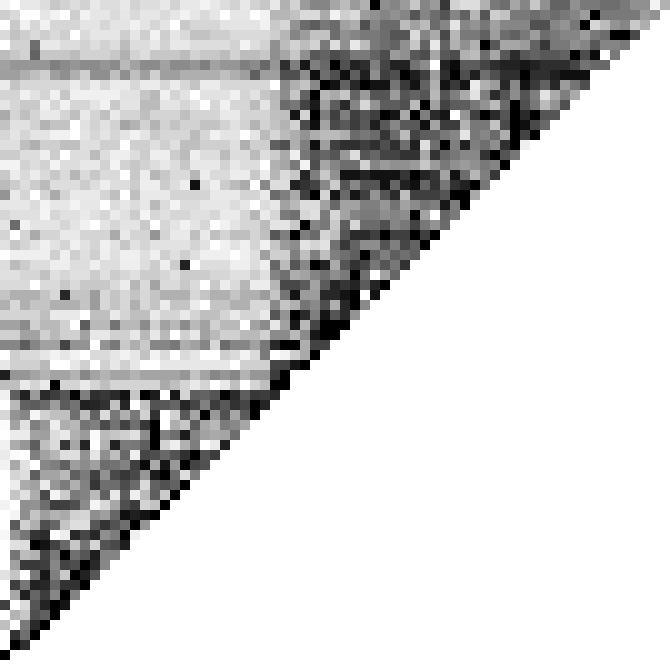
\includegraphics[width=.4\linewidth]{images/odd/max_config23.png}
    \caption{Example of odd CIAO Plot}
    \label{odd}
\end{figure}


Most of the CIAO plots produced throughout all the configurations tended to show \textit{mediocre stability}; which as discussed earlier is just when the two populations no longer evolve.
An example of this plot can be seen in Fig. \ref{mediocre} and more examples can be seen in the appendix in Fig. \ref{ap_med}.

\begin{figure}[H]
    \centering
    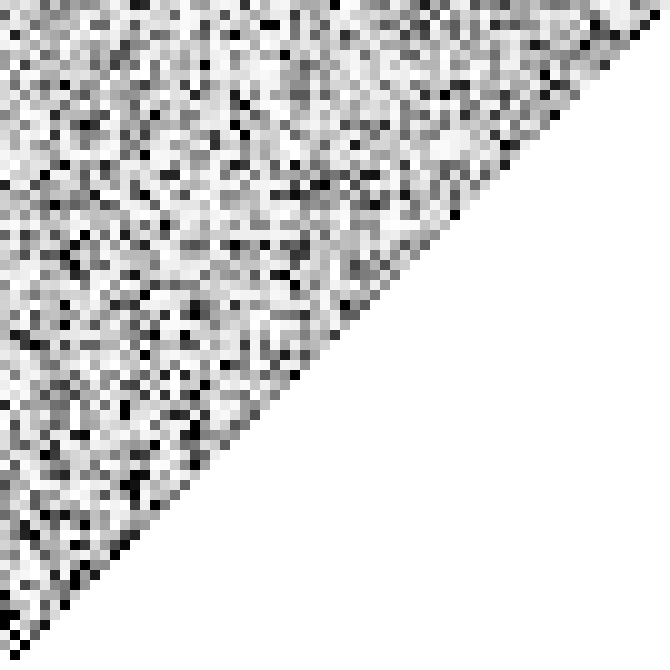
\includegraphics[width=.4\linewidth]{images/mediocre/default_config_16.png}
    \caption{Example of Mediocre Stability}
    \label{mediocre}
\end{figure}

Another issue co-evolution algorithms can exhibit is \textit{cycling}; which did not happen much in these experiments but did happen a few times.
It happened more in the high configuration, which had a pill density of 80\%.
The author is unsure as to why it occur ed in the high configuration more so than the max configuration which had a 100\% pill density. 
Regardless, an example can be seen in Fig. \ref{cycling} with more examples in the appendix in Fig. \ref{ap_cyc}.

\begin{figure}[H]
    \centering
    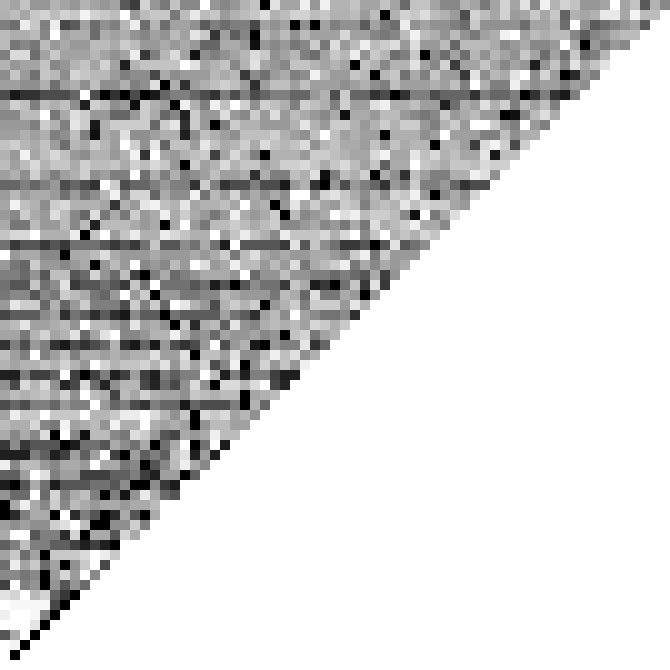
\includegraphics[width=.4\linewidth]{images/cycling/high_config_14.png}
    \caption{Example of Cycling}
    \label{cycling}
\end{figure}

